\documentclass[tikz,border=2pt]{standalone}
\usepackage{amsmath,amssymb}
\usepackage{tikz}
\usetikzlibrary{arrows.meta}

\begin{document}
% Basic solutions of the augmented Giapetto system (5 variables, 3 equations): set 2
% variables to zero and solve for the other 3. Each choice is an intersection of two
% boundary lines — feasible ones are corners, others lie outside.
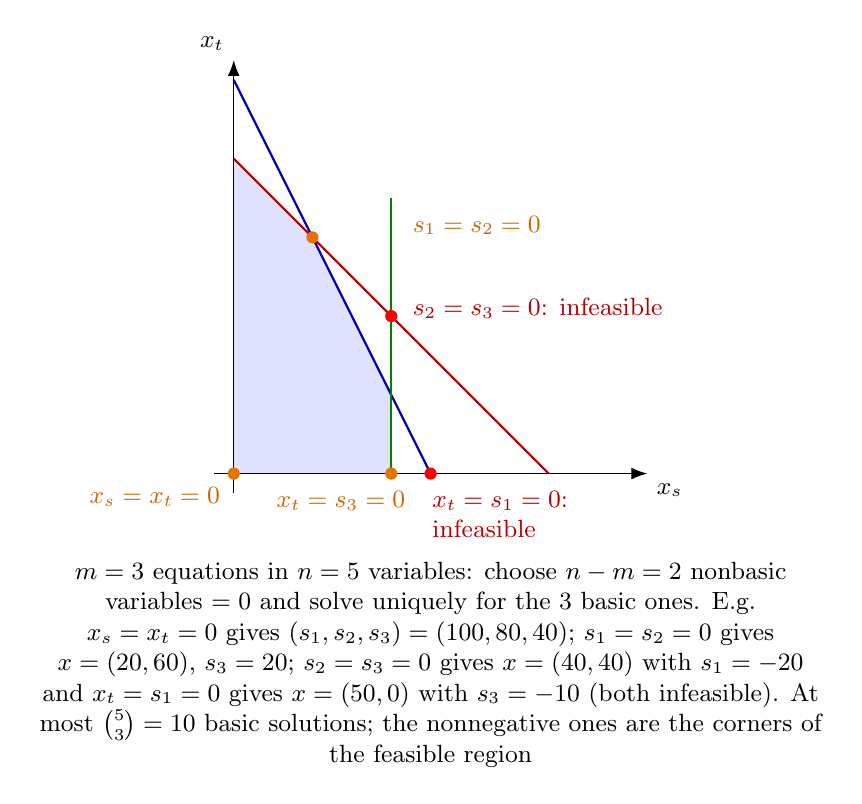
\begin{tikzpicture}[x=0.05cm, y=0.05cm, every node/.style={font=\small}, >={Latex[length=2mm]}]
	\fill[blue!12] (0,0) -- (40,0) -- (40,20) -- (20,60) -- (0,80) -- cycle;
	\draw[->] (-5,0) -- (105,0) node[below right] {$x_s$};
	\draw[->] (0,-5) -- (0,105) node[above left] {$x_t$};
	\draw[blue!70!black, thick] (50,0) -- (0,100);
	\draw[red!70!black, thick] (80,0) -- (0,80);
	\draw[green!50!black, thick] (40,0) -- (40,70);
	\foreach \p in {(0,0),(20,60),(40,0)} {\fill[orange!90!black] \p circle (2.2pt);}
	\foreach \p in {(40,40),(50,0)} {\fill[red] \p circle (2.2pt);}
	\node[orange!80!black, font=\small, anchor=north east] at (-1,-1) {$x_s=x_t=0$};
	\node[orange!80!black, font=\small, anchor=west] at (43,63) {$s_1=s_2=0$};
	\node[orange!80!black, font=\small, anchor=north east] at (46,-2) {$x_t=s_3=0$};
	\node[red!70!black, font=\small, anchor=west] at (43,42) {$s_2=s_3=0$: infeasible};
	\node[red!70!black, font=\small, anchor=north west, align=left] at (48,-2) {$x_t=s_1=0$:\\ infeasible};
	\node[anchor=north, align=flush center, text width=10cm] at (50,-20) {$m=3$ equations in $n=5$ variables: choose $n-m=2$ nonbasic variables $=0$ and solve uniquely for the $3$ basic ones. E.g. $x_s=x_t=0$ gives $(s_1,s_2,s_3)=(100,80,40)$; $s_1=s_2=0$ gives $x=(20,60)$, $s_3=20$; $s_2=s_3=0$ gives $x=(40,40)$ with $s_1=-20$ and $x_t=s_1=0$ gives $x=(50,0)$ with $s_3=-10$ (both infeasible). At most $\binom53=10$ basic solutions; the nonnegative ones are the corners of the feasible region};
\end{tikzpicture}
\end{document}
